\chapter{Related Works}

\section{Data sets}
\subsection{Stanford Sentiment Treebank}
In this thesis, we use Standford Sentiment Treebank (SST) dataset \cite{socher2013recursive}. Standford Sentiment Treebank contains 11,855 sentences. Each data sentence consist of fined-grain sentiment labeled phrases in constituency parse tree structure (see \textbf{Figure \ref{fig:sst}}). There are total 215,154 phrases in whole dataset.
The dataset was splitted into train/dev/test contain 8544/1101/2210 sentences each for training and evaluation models. After remove neutral sentiment sentences, there are 6920/872/1821 sentences remained in train/dev/test set.

SST dataset are publicly available online \footnote{https://nlp.stanford.edu/sentiment/index.html}.

\begin{figure}[H]
	\begin{minipage}{\textwidth}
		\centering
		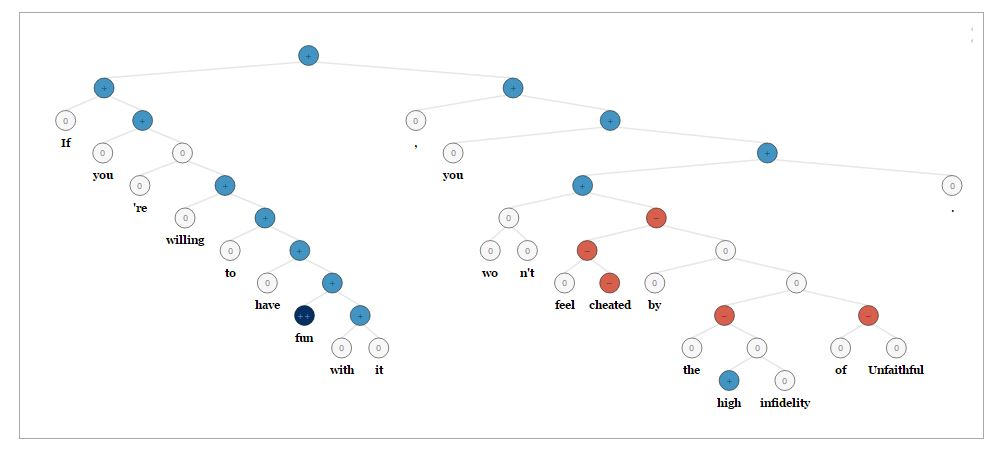
\includegraphics[width=0.9\linewidth]{figure/sst}
		\caption[A parsed sentence in SST]{A parsed sentence in SST \footnote{Render by Pytreebank \url{https://github.com/JonathanRaiman/pytreebank}}}
		\label{fig:sst}
	\end{minipage}
\end{figure}

\footnote{\url{https://github.com/stanfordnlp/treelstm}} to preprocess SST.

\subsection{Julian McAuley's Amazon reviews data set}
We get Amazon Movies and TV reviews (4,607,047 reviews) and Amazon Book reviews (22,507,155 reviews) \cite{he2016ups}. Listing \ref{lst:amzrevie} is sample of one book review.

\begin{lstlisting}[caption={Amazon reviews sample},label={lst:amzreview}]
	{
		"reviewerID": "AH2L9G3DQHHAJ",
		"asin": "0000000116",
		"reviewerName": "chris",
		"helpful": [5, 5],
		"reviewText": "Interesting Grisham tale of a lawyer that takes millions of dollars from his firm after faking his own death. Grisham usually is able to hook his readers early and ,in this case, doesn't play his hand to soon. The usually reliable Frank Mueller makes this story even an even better bet on Audiobook.",
		"overall": 4.0,
		"summary": "Show me the money!",
		"unixReviewTime": 1019865600,
		"reviewTime": "04 27, 2002"
	}
\end{lstlisting}

\subsubsection{Preprocess}
\textbf{Step 1:}
We extract reviewText and overall from review dataset. We assume that overall valus are sentiment score for reviews. Reviews with overall 5 is very positive and 0 is very negative. We keep asin, reviewText, overall and ommit other data points.

\textbf{Step 2:}
We group dataset by product (reviews with same asin). Then for each product, we sorted by overal.

\textbf{Step 3:}
We dump all reviewText into plain text file. We preprocess Standford Tokenizer \cite{tokenizerpart}.

We also make a version of unsorted dataset. We preprocess as we do to our sorted dataset. However, in \textbf{Step 2:}, instead sort review, we suffle all reviews.

\section{Improving sentence composition}
\subsection{Qiao Qian's article on multilayer convolution neural network}
\subsubsection{Method}

\subsubsection{Results and Discussion}


\subsection{Kai Seng Tai's TreeLSTM article}
Compare to other network architects, Recurrent Neural Network have a great advantage in handling sequential, arbitrary length input (e.g. sentences, paragraphs, a sequence of frame in a video or a sequence of acoustic unit in a spoken word) but on the other hand, it also come with the disadvantage of being hard to train.
Given a sequence of input, the network has to capture features which can be long-range relationships between inputs.
One way to improve such structure would be to make these features easier to capture, in other words, shorten the length of relationships between inputs.
For the case of sentence, we can present the it as a syntactic parse tree, in which relevant words and phrases are presented closer to each other in a intuitive way (as human, we understand sentences base on phased and phrases base on words). 
The authors explored this idea by using tree-structured LSTM to combine sentence presentation from its words.
They archive state-of-the-art performance on two tasks: predicting the semantic relatedness of two sentences (SemEval 2014, Task 1) and sentiment classification (Stanford Sentiment Treebank).

Given the advantages of tree structure over it sequential counterpart, we will apply this theory into our model in 4.1.
As we only interested in  the task of sentiment analysis, the experiment and result which related to the task of semantic relatedness will not be presented.

TODO: update 4.1

\subsubsection{Method}
\paragraph{Child-Sum Tree-LSTMs}
Given a tree, we denote \(C(j)\) as set of children of node \(j\).
The step of calculation inside Child-Sum Tree-LSTM node \(j\) can be expressed as follow:
\begin{align}
  	\tilde{h_j} &= \sum_{k \in C(j)} h_k &\label{eq1:2}\\
  	i_j &= \sigma{(W^{(i)}x_j + U^{(i)}\tilde{h_j} + b^{(i)})} &\label{eq1:3}\\
  	f_{jk} &= \sigma{(W^{(f)}x_j + U^{(i)}h_k + b^{(f)})}, \qquad  \forall k \in C(j) & \label{eq1:foget1}\\
  	o_j &= \sigma{(W^{(o)}x_j + U^{(o)}\tilde{h_j} + b^{(o)})} &\label{eq1:5}\\
  	u_j &= \tanh{(W^{(u)}x_j + U^{(u)}\tilde{h_j} + b^{(u)})} &\label{eq1:6}\\
   	c_j &= i_j \odot u_j + \sum_{k \in C(j)} f_{jk} \odot c_k & \\
	h_j &= o_j \odot \tanh{(c_j)} &
\end{align}

As Child-Sum Tree-LSTMs has ability to combine node with arbitrary number of children, it is can be applied to compose sentence bases on it dependency parse tree.
This application was named by the authors as \textbf{Dependency Tree-LSTMs}

\paragraph{N-ary Tree-LSTMs}
Given a tree, we denote \(C(j)\) as set of children of node \(j\) and \(N\) as the maximum number of children a node can have. 
We will assume that the number of child in a node is always \(0\) or \(N\). 
If a node have no children nodes, we call it a leaf-node, else, it will be called a composer-node. 

The step of calculation inside leaf-node \(j\) can be expressed as follow:
\begin{align}
	o_j &= \sigma{\left( W^{(o)} x_j + a^{\left(o\right)}\right)} & \\
   	c_j &= W^{(c)} x_j + a^{(c)} & \\
	h_j &= o_j \odot \tanh{\left(c_j\right)} &
\end{align}

The step of calculation inside composer-node \(j\) can be expressed as follow:
\begin{align}
  	i_j &= \sigma{ \left(\sum_{l=1}^{N}U_l^{(i)} h_{jl} + b^{(i)} \right) } &\label{eq:9}\\
  	f_{jk} &= \sigma{\left(\sum_{l=1}^{N}U_{kl}^{\left(f\right)} h_{jl} + b^{\left(f\right)}\right)}, \qquad  \forall k \in C(j) & \label{eq:foget2}\\ 
  	o_j &= \sigma{\left( \sum_{l=1}^{N}U_l^{\left(o\right)} h_{jl} + b^{\left(o\right)}\right)} &\label{eq:11}\\
  	u_j &= \tanh{\left( \sum_{l=1}^{N}U_l^{\left(u\right)} h_{jl} + b^{\left(u\right)}\right)} &\label{eq:12}\\
   	c_j &= i_j \odot u_j + \sum_{k \in C\left(j\right)} f_{jk} \odot c_{jl} & \\
	h_j &= o_j \odot \tanh{\left(c_j\right)} & \\
\end{align}

Different from Child-Sum Tree-LSTMs forget gate in Eq.\eqref{eq1:foget1}, N-ary Tree-LSTMs chooses what to forget based on all it children as in Eq.\eqref{eq:foget2}. 
Also, each the combination of \(h_{jl}\) in Eqs.\eqref{eq:9},\eqref{eq:11}, \eqref{eq:12} are parameterize by \(U_l^{(i)}\), \(U_l^{(o)}\) and \(U_l^{(u)}\) respectively, compares to linear transformation of sum (\eqref{eq1:2}, \eqref{eq1:3}, \eqref{eq1:5}, \eqref{eq1:6}) in Child-Sum Tree-LSTMs.

Knowing that constituency parse tree can always be presented in binarized form, to compose a sentence the authors applied 2-ary Tree-LSTMs on the binarized constituency parse tree of that sentence. 
This combination was named by the authors as \textbf{Constituency Tree-LSTMs}.

Denoting sequence of words spanned by a sub-tree rooted at node \(j\) as \(\{x\}_j\). 
For both Dependency Tree-LSTMs and Constituency Tree-LSTMs when applying on the task of sentiment analysis, prediction at node \(j\) can be computed by a output-module as follow:

\begin{align}
  	\hat{p_{\theta}}(y \mid \{x\}_j ) &= softmax( W^{(s)} h_j + b^{(s)}) & \\
  	\hat{y_j} &= \underset{y}{\mathrm{argmax}} \; \hat{p_{\theta}}(y \mid \{x\}_j ) &
\end{align}

We use negative log-likelihood with \(L2\) regularization as loss function.

\paragraph{Training technique and hyper-parameters}
Glove vectors was used to initialize word-embedding. 
The words presentation were updated with learning rate 0.1 while other parameters in the network were update using AdaGrad (ref) with learning rate 0.05. 
Batch-size was set to 25. \(L2\) regularization was apply at each mini-batch with weight of \(10^{-4}\).
The authors also added a dropout layer with dropout rate of \(0.5\) before each output-module.

\subsubsection{Results and Discussion}


\subsection{Yoon Kim's article on one layer CNN}
\subsubsection{Method}

\subsubsection{Results and Discussion}


\subsection{Xingyou Wang's article on CRNN}
\subsubsection{Method}

\subsubsection{Results and Discussion}


\section{Improving continuous distributed word presentation}

\subsection{Duyu Tang's article on Twitter word embedding}
\subsubsection{Method}

\subsubsection{Results and Discussion}


\subsection{Misha Denil's article on hierarchical CNN}
\subsubsection{Method}

\subsubsection{Results and Discussion}


\subsection{Dimitrios Kotzias's article on MIL}
\subsubsection{Method}

\subsubsection{Results and Discussion}
